% --------------------------------------------------------------
% This is all preamble stuff that you don't have to worry about.
% Head down to where it says "Start here"
% --------------------------------------------------------------
 
\documentclass[12pt]{article}
 
\usepackage[margin=1in]{geometry} 
\usepackage{amsmath,amsthm,amssymb}
\usepackage{mathtools}
\usepackage{multicol}
\usepackage{textcomp}
\usepackage{float}

\newcommand{\N}{\mathbb{N}}
\newcommand{\Z}{\mathbb{Z}}
\newcommand\aug{\fboxsep=-\fboxrule\!\!\!\fbox{\strut}\!\!\!}
 
\newenvironment{theorem}[2][Theorem]{\begin{trivlist}
\item[\hskip \labelsep {\bfseries #1}\hskip \labelsep {\bfseries #2.}]}{\end{trivlist}}
\newenvironment{lemma}[2][Lemma]{\begin{trivlist}
\item[\hskip \labelsep {\bfseries #1}\hskip \labelsep {\bfseries #2.}]}{\end{trivlist}}
\newenvironment{exercise}[2][Exercise]{\begin{trivlist}
\item[\hskip \labelsep {\bfseries #1}\hskip \labelsep {\bfseries #2.}]}{\end{trivlist}}
\newenvironment{reflection}[2][Reflection]{\begin{trivlist}
\item[\hskip \labelsep {\bfseries #1}\hskip \labelsep {\bfseries #2.}]}{\end{trivlist}}
\newenvironment{proposition}[2][Proposition]{\begin{trivlist}
\item[\hskip \labelsep {\bfseries #1}\hskip \labelsep {\bfseries #2.}]}{\end{trivlist}}
\newenvironment{corollary}[2][Corollary]{\begin{trivlist}
\item[\hskip \labelsep {\bfseries #1}\hskip \labelsep {\bfseries #2.}]}{\end{trivlist}}
 
\begin{document}
 
% --------------------------------------------------------------
%                         Start here
% --------------------------------------------------------------
 
%\renewcommand{\qedsymbol}{\filledbox}
 

% --------------------------------------------------------------
%     You don't have to mess with anything below this line.
% --------------------------------------------------------------
% \title{TUTORIAL 1}%replace X with the appropriate number
\author{TRISTAN GLATARD\\ %replace with your name
COMP 361 Numerial Methods} %if necessary, replace with your course title
\date{September 14, 2018} 
\maketitle

\begin{exercise}{1} %You can use theorem, proposition, exercise, or reflection here.  
By evaluating the determinant, classify the following matrices as singular, ill-conditioned, or well-conditioned:\\
\begin{center}

%A
$\textbf{A}= 
\begin{bmatrix}
1&2&3 \\4&5&6 \\ 7&8&9
\end{bmatrix}$
%B
$\textbf{B}= 
\begin{bmatrix}
2&-2&1 \\1&0&-1 \\ 4&1&1
\end{bmatrix}$
%C
$\textbf{C}= 
\begin{bmatrix}
1&2.0001&3 \\4&5&6 \\ 7&8&9
\end{bmatrix}$
\end{center}
\textbf{Solution}\\

%Calculate det(A)
$
\vert A \vert = 1 
\begin{vmatrix}
5&6 \\ 8&9
\end{vmatrix} - 2
\begin{vmatrix}
4&6 \\ 7&9
\end{vmatrix} + 3
\begin{vmatrix}
4&5 \\ 7&8
\end{vmatrix} = 45 - 48 - 2 (36-42) + 3 (32 - 35) = -3 + 2*6 - 3*3 = 0 
$ 

\textit{A is singular.} \\

%Calculate det(B)
$
\vert B \vert = 2 
\begin{vmatrix}
0&-1 \\ 1&1
\end{vmatrix} + 2
\begin{vmatrix}
1&-1 \\ 4&1
\end{vmatrix} + 1
\begin{vmatrix}
1&0\\4&1
\end{vmatrix}=2*1+2*5+1=13
$ \\

\textit{B is well-conditioned.} \\

%Calculate det(C)
$
\vert C \vert = 1 
\begin{vmatrix}
5&6 \\ 8&9
\end{vmatrix} - 2.0001
\begin{vmatrix}
4&6 \\ 7&9
\end{vmatrix} + 3
\begin{vmatrix}
4&5 \\ 7&8
\end{vmatrix} = -3 + 2.0001*6 - 3*3 = 0.0006 \\
$ \\

As $\vert C \vert << max(c_{ij})$, \textit{C is ill-conditioned.} \\
\end{exercise}

%EXERCISE 2-----------------------------------------------------
\begin{exercise}{2} %You can use theorem, proposition, exercise, or reflection here.  
Find Doolittle's LU decomposition of \textbf{A}:\\
\begin{center}
$\textbf{A}= 
\begin{bmatrix}
2&-2&1\\1&0&-1\\4&1&1
\end{bmatrix}$
\end{center}
\textbf{Solution}\\
Doolittle's decomposition is obtained through Gauss elimination by storing multipliers in the lower part of A \\
$
(2) \longleftarrow (2) - \frac{1}{2} (1)\\
(3) \longleftarrow (3) - 2(1)\\
$
\begin{center}
\textbf{A}= 
$\begin{bmatrix}
2&-2&1\\ 
\boxed{\frac{1}{2}}&1&-\frac{3}{2}\\
\boxed{2}&5&-1
\end{bmatrix}
$ 
\end{center}
$(3) \Leftarrow (3) - 5(2)\\$
\begin{center}
\textbf{[L\textbackslash U]}= 
$\begin{bmatrix}
2&-2&1\\ 
\boxed{\frac{1}{2}}&1&-\frac{3}{2}\\
\boxed{2}&\boxed{5}&\frac{13}{2}
\end{bmatrix}
$ 
\end{center}
Thus,
\begin{center}
\textbf{L}= 
$\begin{bmatrix}
1&0&0\\ 
\frac{1}{2}&1&0\\
2&5&1
\end{bmatrix}
$ 
\textbf{U}= 
$\begin{bmatrix}
2&-2&1\\ 
0&1&-\frac{3}{2}\\
0&0&\frac{13}{2}
\end{bmatrix}
$ 
\end{center}
\end{exercise}

%EXERCISE 3-----------------------------------------------------
\begin{exercise}{3} %You can use theorem, proposition, exercise, or reflection here.  
Using the LU decomposition of $\textbf{A}$ found previously, solve $\textbf{Ax}=\textbf{b}$, where:\\
\begin{center}
\textbf{b}= 
$\begin{bmatrix}
1\\2\\0 
\end{bmatrix}
$ 
\end{center}
\textbf{Solution}\\
1. Solve $Ly = b$ by forward substitution
\begin{itemize}
\item $y_1 = 1$
\item $\frac{1}{2}y_1 + y_2=2 \Rightarrow y_2=\frac{3}{2}$
\item $2y_1+5y_2+y_3=0 \Rightarrow y_3=-\frac{19}{2}$
\end{itemize}
2. Solve $Ux = y$ by forward substitution
\begin{itemize}
\item $\frac{13}{2}x_3=-\frac{19}{2} \Rightarrow x_3=-\frac{19}{13}$
\item $x_2-\frac{3}{2}x_3=\frac{3}{2} \Rightarrow x_2=-\frac{9}{13}$
\item $2x_1-2x_2+x_3=1 \Rightarrow x_1=\frac{1}{2}(1-\frac{18}{13}+\frac{19}{13})=\frac{7}{13}$
\end{itemize}
\end{exercise}
 
%EXERCISE 4-----------------------------------------------------
\begin{exercise}{4} %You can use theorem, proposition, exercise, or reflection here.  
Use Gauss elimination to solve $\textbf{AX}=\textbf{B}$, where:
\begin{center}
\textbf{A}= 
$\begin{bmatrix}
0&1&4\\ 
2&0&7\\
1&0&4
\end{bmatrix}
$ 
\textbf{B}= 
$\begin{bmatrix}
-1&3\\ 6&2\\ 0&1
\end{bmatrix}
$ 
\end{center}
\textbf{Solution}\\
\begin{center}
\textbf{[$A \vert B$]}= 
$\begin{bmatrix}
0&1&4 &\aug&-1&3\\ 
2&0&7 &\aug& 6&2\\
1&0&4 &\aug& 0&1
\end{bmatrix}
$ 
\end{center}
Row 1 needs to be moved, for instance by swapping with Row 2\\
\begin{center}
\textbf{[$A \vert B$]}= 
$\begin{bmatrix}
2&0&7 &\aug& 6&2\\
0&1&4 &\aug&-1&3\\ 
1&0&4 &\aug& 0&1
\end{bmatrix}
$ 
\end{center}
$(3) \leftarrow (3) - \frac{1}{2}(1)$
\begin{center}
\textbf{[$A \vert B$]}= 
$\begin{bmatrix}
2&0&7 &\aug& 6&2\\
0&1&4 &\aug&-1&3\\ 
0&4&-\frac{7}{2} &\aug& -3&0
\end{bmatrix}
$
\end{center}
$(3) \leftarrow (3) - 4(2)$
\begin{center}
\textbf{[$A \vert B$]}= 
$\begin{bmatrix}
2&0&7 &\aug& 6&2\\
0&1&4 &\aug&-1&3\\ 
0&0&-\frac{39}{2} &\aug&1&-12
\end{bmatrix}
$ 
\end{center}
Back substitution
\begin{multicols}{2}
\begin{itemize}
\item $-\frac{39}{2}x_{31} = 1 \Rightarrow x_{31} = -\frac{2}{39}$
\item $x_{21}+4x_{31} = -1 \Rightarrow x_{21} = -\frac{31}{39}$
\item $2x_{11}+7x_{31} = 6 \Rightarrow x_{11} = -\frac{124}{39}$
\end{itemize}
\begin{itemize}
\item $-\frac{39}{2}x_{32} = -12 \Rightarrow x_{32} = \frac{8}{13}$
\item $x_{22}+4x_{32} = 3 \Rightarrow x_{22} = \frac{7}{13}$
\item $2x_{12}+7x_{32} = 2 \Rightarrow x_{12} = -\frac{15}{13}$
\end{itemize}
\end{multicols}
\end{exercise}
%EXERCISE 5-----------------------------------------------------
\begin{exercise}{5} %You can use theorem, proposition, exercise, or reflection here.  
Compute the condition number of $\textbf{A}$ using the infinity norm:
\begin{center}
\textbf{A}= 
$\begin{bmatrix}
2&-2&1\\ 
1&0&-1\\
4&1&1
\end{bmatrix}
$ 
\end{center}
\textbf{Solution}\\

cond(A) = $\Vert A \Vert_\infty . \Vert A^{-1} \Vert_\infty = 6 . \Vert A^{-1} \Vert_\infty$ \\
We need to find $A^{-1}$. We can do it by solving equations $AX = I$ by Gauss elimination. But we already have the LU decomposition of \textbf{A} from \textbf{Excercise 2}: 
\begin{center}
\textbf{L}= 
$\begin{bmatrix}
1&0&0\\ 
\frac{1}{2}&1&0\\
2&5&1
\end{bmatrix}
$ 
\textbf{U}= 
$\begin{bmatrix}
2&-2&1\\ 
0&1&-\frac{3}{2}\\
0&0&\frac{13}{2}
\end{bmatrix}
$ 
\end{center}
Now we need to solve $LUX = I$, where I is the identity matrix:
\begin{center}
$ I = \begin{bmatrix}
1&0&0\\ 
0&1&0\\
0&0&1
\end{bmatrix}
$ 
\end{center}

1. Solve $LUX=\begin{bmatrix} 1\\0\\0\end{bmatrix}$\\

1.1. Solve $Ly=\begin{bmatrix} 1\\0\\0\end{bmatrix}$ by forward substitution
\begin{center}
$y_1 = 1; y_2=-\frac{1}{2};y_3=\frac{1}{2}$
\end{center}

1.2. Solve $Ux=y=\begin{bmatrix} 1\\-\frac{1}{2}\\\frac{1}{2}\end{bmatrix}$
by backward substitution
\begin{center}
$x_3=\frac{1}{13};x_2=-\frac{5}{13};x_1=\frac{1}{13}$
\end{center}

2. Solve $LUX=\begin{bmatrix} 0\\1\\0\end{bmatrix}$

2.1 Solve $Ly=\begin{bmatrix} 0\\1\\0\end{bmatrix}$ by forward substitution
\begin{center}
$y_1 = 0; y_2=1;y_3=-5$
\end{center}

2.2 Solve $Ux=y=\begin{bmatrix} 0\\1\\-5\end{bmatrix}$ by backward substitution
\begin{center}
$x_3=-\frac{10}{13};x_2=-\frac{2}{13};x_1=\frac{3}{13}$
\end{center}

3. Solve $LUX=\begin{bmatrix} 0\\0\\1\end{bmatrix}$

3.1. Solve $Ly=\begin{bmatrix} 0\\0\\1\end{bmatrix}$ by forward substitution
\begin{center}
$y_1 = 0; y_2=0;y_3=1$
\end{center}

3.2. Solve $Ux=y=\begin{bmatrix} 0\\0\\1\end{bmatrix}$ by backward substitution
\begin{center}
$x_3=-\frac{2}{13};x_2=-\frac{3}{13};x_1=\frac{3}{13}$
\end{center}

Finally,
\begin{center}
$A^{-1} = \begin{bmatrix}
\frac{1}{13}&\frac{3}{13}&\frac{2}{13}\\ 
-\frac{5}{13}&-\frac{2}{13}&\frac{3}{13}\\ 
\frac{1}{13}&-\frac{10}{13}&\frac{2}{13}\\ 
\end{bmatrix}
$, and $\Vert A^{-1} \Vert _\infty = 1$ \\
\end{center}

\textbf{cond(A) = 6}
\end{exercise}
%EXERCISE 6-----------------------------------------------------
\begin{exercise}{6} %You can use theorem, proposition, exercise, or reflection here.  
Invert the following matrix:
\begin{center}
\textbf{A}= 
$\begin{bmatrix}
3&1&2\\ 
1&1&0\\
5&8&9
\end{bmatrix}
$ 
\end{center}
\textbf{Solution}\\

We will solve $AX=I$ by Gauss elimination\\
\begin{center}
\textbf{[$A \vert I$]}= 
$\begin{bmatrix}
3&1&2 &\aug&1&0&0\\ 
1&1&0 &\aug& 0&1&0\\
5&8&9 &\aug& 0&0&1
\end{bmatrix}
$ \\
\end{center}
$(2) \leftarrow (2) - \frac{1}{3}(1)$\\
$(3) \leftarrow (3) - \frac{5}{3}(1)$\\
\begin{center}
$\begin{bmatrix}
3&1&2 &\aug&1&0&0\\ 
0&\frac{2}{3}&-\frac{2}{3} &\aug&-\frac{1}{3}&1&0\\
0&\frac{19}{3}&\frac{17}{3} &\aug& -\frac{5}{3}&0&1
\end{bmatrix}
$ \\
\end{center}
$(3) \leftarrow (3) - \frac{19}{2}(2)$\\
\begin{center}
$\begin{bmatrix}
3&1&2 &\aug&1&0&0\\ 
0&\frac{2}{3}&-\frac{2}{3} &\aug&-\frac{1}{3}&1&0\\
0&0&12 &\aug& \frac{3}{2}&-\frac{19}{2}&1
\end{bmatrix}
$ \\
\end{center}

Back substitution
\begin{itemize}
\item $12x_{31} = \frac{3}{2} \Rightarrow x_{31} = -\frac{1}{8}$
\item $\frac{2}{3}x_{21} = -\frac{1}{3} + \frac{2.1}{3.8} \Rightarrow x_{21} = -\frac{3}{8}$
\item $x_{11} = \frac{1}{3}(1+\frac{3}{8}-\frac{2}{8}) = \frac{3}{8}$
\end{itemize}

\begin{itemize}
\item $12x_{32} = -\frac{19}{2} \Rightarrow x_{32} = -\frac{19}{24}$
\item $x_{22} = -\frac{3}{2}(1-\frac{2}{3}.\frac{19}{24}) = -\frac{17}{24}$
\item $x_{12} = \frac{1}{3}(0-\frac{17}{24}+2\frac{19}{24}) = \frac{7}{24}$
\end{itemize}

\begin{itemize}
\item $12x_{33} = 1 \Rightarrow x_{33} = \frac{1}{12}$
\item $x_{23} = -\frac{3}{2}(0+\frac{2}{3}.\frac{1}{12}) = \frac{1}{12}$
\item $x_{13} = \frac{1}{3}(0-\frac{1}{12}-\frac{2}{12}) = -\frac{1}{12}$
\end{itemize}

Finally,
\begin{center}
$A^{-1} = \begin{bmatrix}
\frac{3}{8}&\frac{7}{24}&-\frac{1}{12}\\ 
-\frac{3}{8}&-\frac{17}{24}&\frac{1}{12}\\ 
\frac{1}{8}&-\frac{19}{24}&\frac{1}{12}\\ 
\end{bmatrix}
$
\end{center}
\end{exercise}
%EXERCISE 7-----------------------------------------------------
\begin{exercise}{7} %You can use theorem, proposition, exercise, or reflection here.  
Find the Cholesky decomposition of $\textbf{A}$:
\begin{center}
\textbf{A}= 
$\begin{bmatrix}
1&1&1\\ 
1&2&2\\
1&2&3
\end{bmatrix}
$ 
\end{center}
\textbf{Solution}\\
\begin{center}
$\textbf{A}= LL^T =  
\begin{bmatrix}
L_{11}&0&0\\ 
L_{21}&L_{22}&0\\
L_{31}&L_{32}&L_{33}\\
\end{bmatrix}
\begin{bmatrix}
L_{11}&L_{21}&L_{31}\\ 
0&L_{22}&L_{32}\\
0&0&L_{33}\\
\end{bmatrix}
$ 
\end{center}

Identification of column 1:
\begin{itemize}
\item $L_{11} = 1$
\item $L_{11}L_{21} = 1 \Rightarrow L_{21} = 1$
\item $L_{11}L_{31} = 1 \Rightarrow L_{31} = 1$
\end{itemize}

Identification of column 2:
\begin{itemize}
\item $L_{21}^2 + L_{22}^2 = 2 \Rightarrow L_{22} = 1$
\item $1+L_{22}L_{32} = 2 \Rightarrow L_{32} = 1$
\end{itemize}

Identification of column 3:
\begin{itemize}
\item $L_{31}^2 + L_{32}^2  + L_{33}^2 = 3 \Rightarrow L_{33} = 1$
\end{itemize}

Therefore,
\begin{center}
\textbf{L}= 
$\begin{bmatrix}
1&0&0\\ 
1&1&0\\
1&1&1
\end{bmatrix}
$ 
\end{center}

\end{exercise}
 
% % --------------------------------------------------------------
% This is all preamble stuff that you don't have to worry about.
% Head down to where it says "Start here"
% --------------------------------------------------------------
 

% --------------------------------------------------------------
%                         Start here
% --------------------------------------------------------------
 
%\renewcommand{\qedsymbol}{\filledbox}

\title{TUTORIAL 2}%replace X with the appropriate number
\author{TRISTAN GLATARD\\ %replace with your name
COMP 361 Numerial Methods} %if necessary, replace with your course title
\date{September 21, 2018} 
\maketitle

\begin{exercise}{1} %You can use theorem, proposition, exercise, or reflection here.  
Determine y at x = 0 using Lagrange\textquotesingle s method for the given data points:\\
\begin{table}[h]
\centering
\begin{tabular}{|c|c|c|c|}
\hline
x & -1.2 & 0.3 & 1.1 \\ \hline
y & -5.76 & -5.61 & -3.69 \\ \hline
\end{tabular}
\end{table}

\textbf{Solution.} With 3 given data points, we can construct a degree-2 polynomial using the Lagrange formula:\\
$$P_{2}(x)=\sum_{i=0}^2 y_{i}\ell_{i}(x)$$
where
\begin{align}
\ell_{0}(0)&=\frac{(x-x_1)(x-x_2)}{(x_0-x_1)(x_1-x_2)}=\frac{(0-0.3)(0-1.1)}{(-1.2-0.3)(-1.2-1.1)}&\approx 0.9565 \notag\\
\ell_{1}(0)&=\frac{(x-x_0)(x-x_2)}{(x_1-x_0)(x_1-x_2)}=\frac{(0+1.2)(0-1.1)}{(0.3+1.2)(0.3-1.1)}&= 1.1 \notag\\
\notag 
\ell_{2}(0)&=\frac{(x-x_0)(x-x_1)}{(x_2-x_0)(x_2-x_1)}=\frac{(0+1.2)(0-0.3)}{(1.1+1.2)(1.1-0.3)}&\approx -0.1956
\end{align}
Thus,
\begin{align}
\notag
y(0) = P_{2}(0) &=y_0\ell_0(0) + y_1\ell_2(0) + y_0\ell_2(0)\\ 
\notag
&\approx -5.76*0.9565 + (-5.61)*1.1+(-3.69)(-0.1956) 
\notag
\\&=-10.8726
\notag
\end{align}
\end{exercise}

%EXERCISE 2-----------------------------------------------------
\begin{exercise}{2} %You can use theorem, proposition, exercise, or reflection here.  
Use Newton\textquotesingle s method to find the polynomial that fits the following points:\\
\begin{table}[h]
\centering
\begin{tabular}{|c|c|c|c|c|c|}
\hline
x & -3 & 2 & -1 & 3 & 1 \\ \hline
y & 0 & 5 & -4 & 12 & 0 \\ \hline
\end{tabular}
\end{table}

\textbf{Solution.} Construct the tableau for Newton\textquotesingle s as follow

\begin{table}[H]
\centering
\begin{tabular}{|c|c|c|c|c|c|c|}
\hline
\textit{i} & $x_i$ & $y_i$ & $\nabla y_i$ & $\nabla ^2 y_i$ & $\nabla ^3 y_i$ & $\nabla ^4 y_i$ \\ \hline
0 & -3 & \textbf{0} &  &  &  &  \\ \hline
1 & 2 & 5 & \textbf{1} &  &  &  \\ \hline
2 & -1 & -4 & -2 & \textbf{1} &  &  \\ \hline
3 & 3 & 12 & 2 & 1 & \textbf{0} &  \\ \hline
4 & 1 & 0 & 0 & 1 & 0 & \textbf{0} \\ \hline
\end{tabular}
\end{table}

where elements are calculated as:\\
\begin{align}
\notag
\nabla y_1 &= \frac{y_1-y_0}{x_1-x_0}=\frac{5-0}{2+3}=1\\
\notag
\nabla y_2 &= \frac{y_2-y_0}{x_2-x_0}=\frac{-4+0}{-1+3}=-2\\
\notag
\nabla y_3 &= \frac{y_3-y_0}{x_3-x_0}=\frac{12-0}{3+3}=2\\
\notag
\nabla y_4 &= \frac{y_4-y_0}{x_4-x_0}=0\\
\notag
\nabla ^2 y_2 &= \frac{\nabla y_2-\nabla y_1}{x_2-x_1}=\frac{-2-1}{-1-2}=1\\
\notag
\nabla ^2 y_3 &= \frac{\nabla y_3-\nabla y_1}{x_3-x_1}=\frac{2-1}{3-2}=1\\
\notag
\nabla ^2 y_4 &= \frac{\nabla y_4-\nabla y_1}{x_4-x_1}=\frac{0-1}{1-2}=1\\
\notag
\nabla ^3 y_3 &= \frac{\nabla ^2 y_3-\nabla ^2 y_2}{x_3-x_2}=0\\
\notag
\nabla ^3 y_4 &= \frac{\nabla ^2 y_4-\nabla ^2 y_2}{x_4-x_2}=0\\
\notag
\nabla ^4 y_4 &= \frac{\nabla ^3 y_4-\nabla ^3 y_3}{x_4-x_3}=0\\
\notag
\end{align}
From the tableau \textquotesingle s diagonal, we have\\
\begin{align}
\notag
a_0&=y_0=0\\
\notag
a_1&=\nabla y_1=1\\
\notag
a_2&=\nabla ^2 y_2=1
\end{align}
and the polynomial fit is degree-2 (parabolic).
Evaluate backward with recurrence relations:
\begin{align}
\notag
P_0(x) &= a_2 = 1\\
\notag
P_1(x) &= a_1 + (x-x_1)P_0(x) = 1 + (x-2) = x-1\\
\notag
P_2(x) &= a_0 + (x-x_0)P_1(x) = 0 + (x+3)(x-1) = x^2+2x-3\\
\notag
\end{align}
\end{exercise}

%EXERCISE 2-----------------------------------------------------
\begin{exercise}{3} %You can use theorem, proposition, exercise, or reflection here.  
Use linear regression to find the line that fits the following data and determine the standard deviation:\\
\begin{table}[h]
\centering
\begin{tabular}{|c|c|c|c|c|c|}
\hline
x & -1.0 & -0.5 & 0 & 0.5 & 1.0 \\ \hline
y & -1.00 & -0.55 & 0.00 & 0.45 & 1.00 \\ \hline
\end{tabular}
\end{table}

\textbf{Solution.} With linear regression, we try to fit the data into a line of form
\begin{align}
f(x)=a+bx
\end{align}
where parameters a, b are given as
\begin{align}
b&=\frac{\sum\limits_{i=0}^{n} y_i(x_i-\overline{x})}{\sum\limits_{i=0}^{n} x_i(x_i-\overline{x})}\\
a&=\overline{y}-\overline{x}b
\end{align}

From the data:
\begin{align}
\notag
\overline{x}&=\frac{\sum\limits_{i=0}^{n} x_i}{n+1} = \frac{-1.0-0.5+0+0.5+1.0}{5} = 0 \\
\notag
\overline{y}&=\frac{\sum\limits_{i=0}^{n} y_i}{n+1}= \frac{-1.00 - 0.55 + 0.00 + 0.45 + 1.00}{5} = -0.02
\end{align}
Apply to (2) and (3)
\begin{align}
\notag
b&= \frac{(-1.00)(-1.0) + (-0.55)(-0.5) + 0.00*0 + 0.45*0.5 + 1.00*1.0}{(-1.0)(-1.0)+(-0.5)(-0.5)+0*0+0.5*0.5+1.0*1.0} = \frac{2.5}{2.5} = 1\\
\notag
a&=-0.02-0*1=-0.02
\end{align}
Then (1) becomes
\begin{align}
\notag
f(x)=-0.02 + x
\end{align}
We start the evaluation of the standard deviation by computing the residuals:
\begin{table}[h]
\centering
\begin{tabular}{|c|c|c|c|c|c|}
\hline
x & -1.0 & -0.5 & 0 & 0.5 & 1.0 \\ \hline
y & -1.00 & -0.55 & 0.00 & 0.45 & 1.00 \\ \hline
f(x) & -1.02 & -0.52 & -0.02 & 0.48 & 0.98 \\ \hline
y - f(x) & 0.02 & -0.03 & 0.02 & -0.03 & 0.02 \\ \hline
\end{tabular}
\end{table}
The sum of the squares of the residuals is
\begin{align}
\notag
S&=\sum\limits_{i=0}^4 [y_i-f(x_i)]^2\\
\notag
 &=(0.02)^2 + (-0.03)^2 + (0.02)^2 + (-0.03)^2 + (0.02)^2\\
 \notag
 &=0.003
\end{align}
The standard deviation is given as
\begin{align}
\notag
\sigma=\sqrt[]{\frac{S}{n-m}}
\end{align}
where $S$ is the sum of the squares of the residuals calculated above, $n + 1$ is the number of data points (i.e., $n = 4$), $m$ is the degree of the polynomial (1 in this case, since we fit linear regression)\\
Finally,
\begin{align}
\notag
\sigma=\sqrt[]{\frac{0.003}{4-1}} \approx 0.0316 
\end{align}
\end{exercise}
\begin{exercise}{4} %You can use theorem, proposition, exercise, or reflection here.  
Determine the natural cubic spline that passes through the data points:\\
\begin{table}[h]
\centering
\begin{tabular}{|c|c|c|c|}
\hline
x & 0 & 1 & 2 \\ \hline
y & 0 & 2 & 1 \\ \hline
\end{tabular}
\end{table}

Note that the interpolant consists of two cubics, one valid in $0 \leq x \leq 1$, the other in $1 \leq x \leq 2$. Verify that these cubics have the same first and second derivatives at $x = 1$.

\textbf{Solution.} With 3 given data points, we want to construct two cubics of the form:
\begin{align}
\notag
f_{0,1}(x) &= a_0x^3 + b_0x^2 + c_0x+d_0\\
\notag
f_{1,2}(x) &= a_1x^3 + b_1x^2 + c_1x+d_1
\end{align}

Interpolation gives us
\begin{align}
f_{0,1}(0) = 0 \Rightarrow d_0 = 0\\
f_{0,1}(1) = 2 \Rightarrow a_0 + b_0 + c_0 + d_0 = 2\\
f_{1,2}(1) = 2 \Rightarrow a_1 + b_1 + c_1 + d_1 = 2\\
f_{1,2}(2) = 1 \Rightarrow 8a_1 + 4b_1 + 2c_1 + d_1 = 1
\end{align}

The derivatives of these cubics are:
\begin{align}
\notag
f\prime_{0,1}(x) &= 3a_0x^2 + 2b_0x + c_0\\
\notag
f\prime_{1,2}(x) &= 3a_1x^2 + 2b_1x + c_1
\end{align}

The slope continuity condition gives us
\begin{align}
\notag
f\prime_{0,1}(1) &= f_{1,2}\prime(1)\\
3a_0 + 2b_0 + c_0 &= 3a_1 + 2b_1 + c_1
\end{align}

The second derivatives of these cubics are:
\begin{align}
\notag
f\prime\prime_{0,1}(x) &= 6a_0x + 2b_0\\
\notag
f\prime\prime_{1,2}(x) &= 6a_1x + 2b_1
\end{align}

The boundary conditions of natural spline give us
\begin{align}
f\prime\prime_{0,1}(0) &= 2b_0 = 0\\
f\prime\prime_{1,2}(2) &= 12a_1 + 2b_1 = 0
\end{align}

The continuity of second derivatives gives us
\begin{align}
\notag
f\prime\prime_{0,1}(1) &= f\prime\prime_{1,2}(1)\\
 6a_0 + 2b_0 &= 6a_1 + 2b_1
\end{align}

Solving the system of 8 equations with 8 unknowns gives us \\
$$a_0=-\frac{3}{4},b_0=0,c_0=\frac{11}{4},d_0=0$$\\
$$a_1=\frac{3}{4},b_1=-\frac{9}{2},c_1=\frac{29}{4},d_1=-\frac{3}{2}$$

It is easy to verify that $f\prime\prime_{0,1}(1) = f\prime\prime_{1,2}(1)$
\begin{align}
\notag
f\prime\prime_{0,1}(1) &= 6a_0 + 2b_0 = -\frac{9}{2}\\
\notag
f\prime\prime_{1,2}(1) &= 6a_1 + 2b_1 = -\frac{9}{2}
\end{align}

\textbf{Another solution (a shortcut)}

The three knots are equally spaced at h = 1. Recalling that the second
derivative of a natural spline is zero at the first and last knot, we have $k_0 = k_2 = 0$. 

The second derivatives at the second knot is obtained from Eq. (3.12) in the textbook:
$$k_{i-1}+4k_i+k_{i+1}=\frac{6}{h^2}(y_{i-1}-2y_i+y_{i+1}), i=1,2,...n-1$$

Using i = 1 results in
$$k_0+4k_1+k_2=6(y_0-2y_1+y_2)$$
$$k_1=-\frac{9}{2}$$

Now we can construct the cubics by applying Eq. (3.10) in the textbook:
\begin{align}
\notag
f_{i,i+1}(x) &= \frac{k_i}{6}\left[\frac{(x-x_{i+1})^3}{x_i-x_{i+1}}-(x-x_{i+1})(x_i-x_{i+1})\right]\\ 
\notag
& - \frac{k_{i+1}}{6}\left[\frac{(x-x_i)^3}{x_i-x_{i+1}}-(x-x_i)(x_i-x_{i+1})\right]\\ 
\notag
& + \frac{y_i(x-x_{i+1})-y_{i+1}(x-x_i)}{x_i-x_{i+1}}
\end{align}

With i=0,1 we have two cubics:
\begin{align}
\notag
f_{0,1}(x) &= - \frac{k_1}{6}\left[\frac{(x-x_0)^3}{x_0-x_1}-(x-x_0)(x_0-x_1)\right]
+ \frac{y_0(x-x_1)-y_1(x-x_0)}{x_0-x_1}\\
\notag
&=\frac{3}{4}\left[\frac{x^3}{0-1} - (x-1)(0-1)\right] - \frac{2x}{-1}\\
\notag
&= -\frac{3}{4}x^3 + \frac{11}{4}x\\ 
\notag
f_{1,2}(x) &=\frac{k_1}{6}\left[\frac{(x-x_2)^3}{x_1-x_2}-(x-x_2)(x_1-x_2)\right]
+\frac{y_1(x-x_2)-y_2(x-x_1)}{x_1-x_2}\\
\notag
&=-\frac{3}{4}\left[\frac{(x-2)^3}{1-2} - (x-2)(1-2)\right] - \frac{2(x-2)-(x-1)}{1-2}\\
\notag
&=\frac{3}{4}x^3-\frac{9}{2}x^2+\frac{29}{4}x-\frac{3}{2}
\end{align}
\end{exercise}


% --------------------------------------------------------------
%     You don't have to mess with anything below this line.
% --------------------------------------------------------------
 
\end{document}
 
% --------------------------------------------------------------
% This is all preamble stuff that you don't have to worry about.
% Head down to where it says "Start here"
% --------------------------------------------------------------
 

% --------------------------------------------------------------
%                         Start here
% --------------------------------------------------------------
 
%\renewcommand{\qedsymbol}{\filledbox}

\title{TUTORIAL 4}%replace X with the appropriate number
\author{TRISTAN GLATARD\\ %replace with your name
COMP 361 Numerial Methods} %if necessary, replace with your course title
\date{October 5, 2018} 
\maketitle

\begin{exercise}{1} %You can use theorem, proposition, exercise, or reflection here. 
Draw a plot of $f(x) = cosh(x)cos(x)-1$ in the range $0 \leq x \leq 10$. (a) Verify from the
plot that the smallest positive, nonzero root of $f(x)=0$ lies in the interval (4, 5).
(b) Show graphically that the Newton-Raphson formula would not converge to
this root if it is started with $x = 4$.

\textbf{Solution.} 

Plot of the function is done with Google's help. \textit{Hint: just type the function in Google, it will draw the plot.}

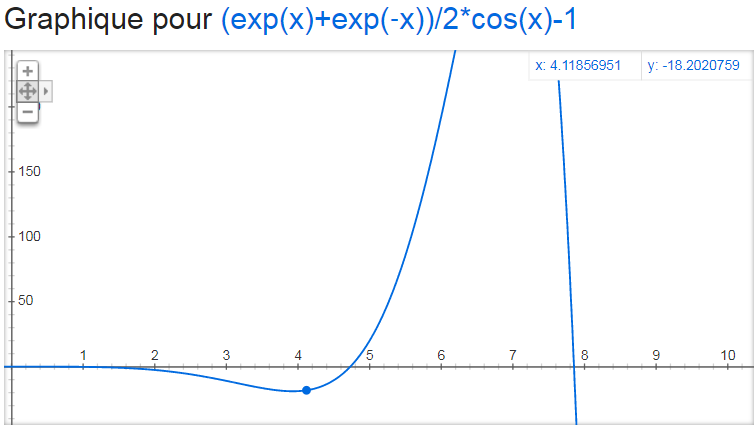
\includegraphics[]{coshxcosx-1.png}

In this plot, we can see that if we start Newton-Raphson method with x=4, the approximation will be out of range [4,5] ($\approx  10.66$, try to verify this!). This is because the approximation is calculated by the tangent line which is not sloppy at $x=4$. (Try to verify this! Hint: the slope of the tangent line at $x_0$ is  $f^\prime(x_0)$. Compare $f^\prime(4)$ and $f^\prime(5)$ )

\end{exercise}

%EXERCISE 2-----------------------------------------------------
\begin{exercise}{2} %You can use theorem, proposition, exercise, or reflection here.  
A zero $x = r$ of $P_n(x)$ is given. Verify that r is indeed a zero, and then deflate the polynomial; that is, find $P_{n-1}(x)$ so that $P_n(x) = (x-r)P_{n-1}(x)$.
\begin{align}
1. P_3(x) &= 3x^3 + 7x^2 - 36x + 20, r = -5 \notag \\
2. P_4(x) &= x^4 - 3x^2 + 3x - 1, r = 1 \notag
\end{align}

\textbf{Solution.}

1. First, verify r = -5 is indeed a zero
\begin{align}
P_3(-5) &= 3*(-5)^3 + 7*(-5)^2 - 36*(-5) + 20 \notag \\
&=-3*125 + 7*25 + 180 + 20 = 0 \notag 
\end{align}

The coefficients of $P_3(x)$ are:
\begin{align}
a_3 = 3, a_2 = 7, a_1 = -36, a_0 = 20 \notag 
\end{align}

Now the deflation of $P_3(x)$ is done as: 
\begin{align}
b_2 &= a_3 = 3 \notag \\ 
b_1 &= a_2 + rb_2 = 7 + (-5)*3 = -8 \notag \\
b_0 &= a_1 + rb_1 = -36 + (-5)(-8) = 4 \notag 
\end{align}

And the deflated polynomial is
\begin{align}
P_2(x) &= 3x^2 - 8x + 4 \notag 
\end{align}

2. First, verify r = 1 is indeed a zero
\begin{align}
P_4(1) &= (1)^4 - 3*1^2 + 3* 1 - 1 \notag \\
&= 0 \notag
\end{align}

The coefficients of $P_4(x)$ are:
\begin{align}
a_4 = 1, a_3 = 0, a_2 = -3, a_1 = 3, a_0 = -1 \notag 
\end{align}

Now the deflation of $P_4(x)$ is done as: 
\begin{align}
b_3 &= a_4 = 1 \notag \\ 
b_2 &= a_3 + rb_3 = 0 + 1*1 = 1 \notag \\ 
b_1 &= a_2 + rb_2 = -3 + 1*1 = -2 \notag \\
b_0 &= a_1 + rb_1 = 3 + 1*(-2) = 1 \notag
\end{align}


And the deflated polynomial is
\begin{align}
P_3(x) &= x^3 + x^2 - 2x + 1 \notag 
\end{align}
\end{exercise}


%EXERCISE 2-----------------------------------------------------
\begin{exercise}{3} %You can use theorem, proposition, exercise, or reflection here.  
A zero $x = r$ of $P_n(x)$ is given.Determine all the other zeros of $P_n(x)$ by
using a calculator. You should need no tools other than deflation and the quadratic
formula.
\begin{align}
1. P_3(x) &= x^3+1.8x^2-9.01x-13.398, r =-3.3\\
2. P_3(x) &= x^3-6.64x^2+16.84x-8.32, r = 0.64
\end{align}

\textbf{Solution.} 

\textbf{Reminder}: the quadratic equation of the form $ax^2 + bx +c = 0$ has two roots:
\begin{align}
x_{1,2} = \frac{-b \pm \sqrt[]{\Delta}}{2a}
\end{align}

where $\Delta = b^2 - 4ac$ 

1. The coefficients of $P_3(x)$ are:
\begin{align}
a_3 = 1, a_2 = 1.8, a_1 = -9.01, a_0 = -13.398 \notag 
\end{align}

Now the deflation of $P_3(x)$ is done as: 
\begin{align}
b_2 &= a_3 = 1 \notag \\ 
b_1 &= a_2 + rb_2 = 1.8 + (-3.3)*1 = -1.5 \notag \\
b_0 &= a_1 + rb_1 = -9.01 + (-3.3)(-1.5) = -4.06 \notag 
\end{align}

And the deflated polynomial is
\begin{align}
P_2(x) &= x^2 - 1.5x - 4.06 \notag 
\end{align}


The above quadratic has two roots, as shown in (3): 
\begin{align}
x_{1,2} &= \frac{1.5 \pm \sqrt[]{1.5^2+4*4.06}}{2} \notag \\
x_1 &= -1.4 \notag \\
x_2 &= 2.9 \notag
\end{align}

2. The coefficients of $P_3(x)$ are:
\begin{align}
a_3 = 1, a_2 = -6.64, a_1 = 16.84, a_0 = -8.32 \notag 
\end{align}


Now the deflation of $P_3(x)$ is done as: 
\begin{align}
b_2 &= a_3 = 1 \notag \\ 
b_1 &= a_2 + rb_2 = -6.64 + 0.64*1 = -6 \notag \\
b_0 &= a_1 + rb_1 = 16.84 + 0.64*(-6) = 13 \notag 
\end{align}


And the deflated polynomial is
\begin{align}
P_2(x) &= x^2 - 6x + 13 \notag 
\end{align}



The above quadratic has two roots as shown in (3): 
\begin{align}
x_{1,2} &= \frac{6 \pm \sqrt[]{6^2-4*13}}{2} \notag \\
&=3 \pm \sqrt[]{-4} \notag \\
&= 3 \pm 2i \notag \\
x_1 &= 3 + 2i \notag \\
x_2 &= 3 - 2i \notag
\end{align}
\end{exercise}
% --------------------------------------------------------------
%     You don't have to mess with anything below this line.
% --------------------------------------------------------------
 
\end{document}
 
\end{document}